\let\negmedspace\undefined
\let\negthickspace\undefined
\documentclass[journal]{IEEEtran}
\usepackage[a5paper, margin=10mm, onecolumn]{geometry}
%\usepackage{lmodern} % Ensure lmodern is loaded for pdflatex
\usepackage{tfrupee} % Include tfrupee package

\setlength{\headheight}{1cm} % Set the height of the header box
\setlength{\headsep}{0mm}     % Set the distance between the header box and the top of the text

\usepackage{gvv-book}
\usepackage{gvv}
\usepackage{cite}
\usepackage{amsmath,amssymb,amsfonts,amsthm}
\usepackage{algorithmic}
\usepackage{graphicx}
\usepackage{textcomp}
\usepackage{xcolor}
\usepackage{txfonts}
\usepackage{listings}
\usepackage{enumitem}
\usepackage{mathtools}
\usepackage{gensymb}
\usepackage{comment}
\usepackage[breaklinks=true]{hyperref}
\usepackage{tkz-euclide} 
\usepackage{listings}
% \usepackage{gvv}                                        
\def\inputGnumericTable{}                                 
\usepackage[latin1]{inputenc}                                
\usepackage{color}                                            
\usepackage{array}                                            
\usepackage{longtable}                                       
\usepackage{calc}                                             
\usepackage{multirow}                                         
\usepackage{hhline}                                           
\usepackage{ifthen}                                           
\usepackage{lscape}
\begin{document}

\bibliographystyle{IEEEtran}
\vspace{3cm}

\title{9.2.1}
\author{EE24BTECH11012 - Bhavanisankar G S}
% \maketitle
% \newpage
% \bigskip
{\let\newpage\relax\maketitle}

\renewcommand{\thefigure}{\theenumi}
\renewcommand{\thetable}{\theenumi}
\setlength{\intextsep}{10pt} % Space between text and floats


\numberwithin{equation}{enumi}
\numberwithin{figure}{enumi}
\renewcommand{\thetable}{\theenumi}

\textbf{LAPLACE TRANSFORMS} \\
\begin{itemize}
	\item Transformation applied on a function results in a function of another variable, unlike an operation which when applied on a function yields another function but of the same variable.
	\item Laplace transform is a very useful technique used to solve complex equations using \textbf{integral transformations}.
	\item Any equation of the form $\int_{a}^{b} f(t) K(p,t) dt = F(p)$ is called an integral transformation, and the function $K(p,t)$ is called the \textbf{Kernel function}. \\
		When $a = 0 \text{ and } b = \infty$, then the integral transformation is called the Laplace transformation.
	\item Notation : Laplace transform of a function $f(x)$ is denoted as $\mathcal{L} \brak{f(x)}$, i.e., $$\mathcal{L} \brak{f(x)} = F(s) = \int_{0}^{\infty} f(x) e^{-sx} dx $$.
	\item It is a linear transformation, since integration is a linear operation.
	\item Laplace transform of some functions : 
		\begin{align}
			f(x) = 0 &\implies F(s) = 0 \\
			f(x) = 1 &\implies F(s) = \frac{1}{s} \\
			f(x) = x^n &\implies F(s) = \frac{n!}{s^{n+1}} \\
			f(x) = e^{at} &\implies F(s) = \frac{1}{s-a} \\
			f(x) = \sin{ax} &\implies F(s) = \frac{a}{s^2 + a^2} \\
			f(x) = \cos{ax} &\implies F(s) = \frac{s}{s^2 + a^2}
		\end{align}
	\item Some other useful results include :
		\begin{align}
			\mathcal{L} \brak{f^{\prime}(x)} &= s F(s) - f(0^{-}) \\
			\mathcal{L} \brak{f^{\prime}(x)} &= s^2 F(s) - s f(0^{-}) - f^{\prime}(0^{-})
		\end{align}
\end{itemise}
\newpage

\textbf{QUESTION}:\\
Consider the differential equation $\frac{d^2 y}{d x^2} - \frac{dy}{dx} = 0$. Verify that $y = e^x + 1$ is a solution for it. \\
\textbf{SOLUTION}: \\
%\input{tables/table.tex} \\ \\ \\
Consider the differential equation, 
$$ \frac{d^2 y}{d x^2} - \frac{dy}{dx} = 0 $$
Applying Laplace transform on both sides, we have \\
\begin{align}
	\mathcal{L} \brak{\frac{d^2 y}{d x^2} - \frac{dy}{dx}} &= \mathcal{L} \brak{0} \\
	\mathcal{L} \brak{\frac{d^2 y}{d x^2}} - \mathcal{L} \brak{\frac{dy}{dx}} &= \mathcal{L} \brak{0} \\
	\brak{s^2 F(s) - s f(0^{-}) - f^{\prime}(0^{-})} - \brak{s F(s) - f(0^{-})} &= 0 \\
	F(s) \brak{s^2 - s} - f(0^{-}) \brak{s-1} - f^{\prime}(0^{-}) &= 0 \\
	F(s) &= \frac{f(0^{-}) \brak{s-1} + f^{\prime}(0^{-})}{s^2 - s} \\
	\mathcal{L} \brak{f(x)} &= \frac{f(0^{-}) - f^{\prime}(0^{-})}{s} + \frac{f^{\prime}(0^{-})}{s-1} \\
	\brak{f(x)} &= \mathcal{L}^{-1} \brak{\frac{f(0^{-}) - f^{\prime}(0^{-})}{s} + \frac{f^{\prime}(0^{-})}{s-1}} \\
	\implies \brak{f(x)} &= \brak{f(0^{-}) - f^{\prime}(0^{-})} \mathcal{L}^{-1} \brak{\frac{1}{s}} + f^{\prime}(0^{-}) \mathcal{L}^{-1} \brak{\frac{1}{s-1}} \\
	f(x) &= \brak{f(0^{-}) - f^{\prime}(0^{-})} + f^{\prime}(0^{-}) e^{x}
\end{align}
When $f^{\prime}(0^{-}) = 1 \text{ and } f(0^{-}) = 2$, we have $y = e^x + 1$, which is the required solution. \\
Hence verified.

\begin{figure}[h]
				 \centering
				 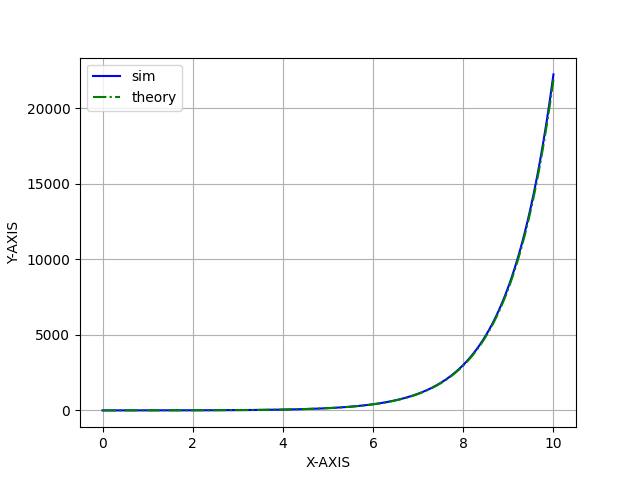
\includegraphics[width=\columnwidth]{figs/fig.png}
				 \caption{A plot of the given question.}
				 \label{fig:Plot1}
			 \end{figure}


\end{document}
